% based on a template made by the university of cologne
% http://www.mi.uni-koeln.de/wp-MIEDV/wp-content/uploads/2016/07/LaTeX-Vorlage.zip - 2023-11-02
\documentclass[12pt,a4paper]{scrartcl}

\addtokomafont{sectioning}{\rmfamily}
\usepackage[ngerman]{babel}% deutsches Sprachpaket wird geladen
\usepackage[T1]{fontenc} % westeuropäische Codierung wird verlangt
\usepackage[utf8]{inputenc}% Umlaute werden erlaubt
\usepackage[usenames]{color} % Erlaubt die Benutzung der namen im Farbpaket und deren Änderung
\usepackage{amsmath} % Erweiterung für den Mathe-Satz
\usepackage{amssymb} % alle Zeichen aus msam und msmb werden dargestellt
\usepackage{graphicx} % Graphiken und Bilder können eingebunden werden
%\usepackage{multirow} % erlaubt in einer Spalte einer Tabelle die Felder in mehreren Zeilen zusammenzufassen
\usepackage{enumerate} % erlaubt Nummerierungen
\usepackage{xurl} % Dient zur Auszeichnung von URLs; setzt die Adresse in Schreibmaschinenschrift.
\usepackage[center]{caption}  % Bildunterschrift wird zentriert
%\usepackage{subfigure} % mehrere Bilder können in einer fugure-Umgebung verwendet werden
%\usepackage{longtable} % Diese Umgebung ist ähnlich definiert wie die tabular-Umgebung, erlaubt jedoch mehrseitige Tabellen.
%\usepackage{paralist} % Modifikation der bereits bestehenden Listenumgebungen
\usepackage{lmodern}% Für die Schrift
\usepackage[hidelinks]{hyperref} % Links und Verweise werden innerhalb von PDF Dokumenten erzeugt
%\usepackage{wrapfig} % Das Paket ermöglicht es von Schrift umflossene Bilder und Tabellen einzufügen.
\usepackage{latexsym} % LaTeX-Symbole werden geladen
\usepackage{tikz} % Erlaubt es mit tikz zu zeichnen
\usepackage{tabularx} % Erlaubt Tabellen
\usepackage{algorithm} % Erlaubt Pseudocode
\usepackage{color} % Farbpaket wird geladen
%\usepackage{stmaryrd} % St Mary Road Symbole werden geladen
\usepackage{physics}
\usepackage{mhchem} % Chemie: \ce & \pu

\numberwithin{equation}{section} % Nummerierungen der Gleichungen, die durch equation erstellt werden, sind gebunden an die section
\newcommand{\HRule}{\rule{\linewidth}{0.7mm}}
\newcommand{\pu}[1]{\ensuremath{\mathrm{#1}}}

% disable commands
\renewcommand{\[}{} % math block start
\renewcommand{\]}{\noindent} % math block end

\hypersetup{
  pdftitle={B1.1},
  pdfcreator={LaTeX via pandoc}}

\setcounter{secnumdepth}{6}
\setcounter{tocdepth}{6}

\begin{document}
\begin{titlepage}
	\pagestyle{empty}

	\begin{center}

	\textsc{\LARGE Universität zu Köln }\\ [0.4cm]
	\textsc{Mathematisch-Naturwissenschaftliche Fakultät} \\[1.5cm]

	
\includegraphics[width=0.45\textwidth]{../media/uni.jpg}\\[1.5cm]  % Uni-Logo wird geladen

	\textsc{\Large Praktikum~B}\\[2mm]
	\textsc{}\\[10mm]
	\HRule \\[0.4cm]

		{	\Huge \bfseries B1.1}\\[0.4cm]
			{	\huge \bfseries Infrarotabsorption in \(\ce{CO_2}\)}\\[0.3cm]
	
	\HRule \\[3cm]

 	\begin{center}
		\textsc{\Large Catherine~Tran } \\[3pt]
		\textsc{\Large Carlo~Kleefisch } \\[3pt]
		\textsc{\Large Oliver~Filla } \\[3pt]
	\end{center}
	\end{center}
\end{titlepage}

\newpage
\tableofcontents
\newpage

\hypertarget{einleitung}{%
\section{Einleitung}\label{einleitung}}

Mithilfe von Spektroskopie ist es möglich, Absorptions- und
Emissionsspektren von elektromagnetischen Wellen an einer Probe zu
beobachten. Hierzu misst man spezifische Größen in Abhängigkeit von der
Frequenz. Dadurch ist es möglich, Aussagen über die mikroskopischen
Eigenschaften der Probe zu treffen.

Alternativ zur Frequenz werden auch äquivalente Größen wie der
Wellenlänge oder Energie verwendet, um Größen wie die Intensität, die
Strahlungsleistung und die Zählrate der Strahlung zu messen.

Dieser Versuch dient als Einführung in die Infrarotspektroskopie.
Mithilfe eines niedrig auflösenden Absorptionsspektrometers wird die
Infrarot--Absorption von Kohlenstoffdioxid \((\ce{CO_2})\) untersucht.
Dieses Gas gehört zu den sogenannten ``Treibhausgasen''.

\clearpage
\hypertarget{theoretische-grundlagen}{%
\section{Theoretische Grundlagen}\label{theoretische-grundlagen}}

\hypertarget{elektromagnetisches-spektrum}{%
\subsection{elektromagnetisches
Spektrum}\label{elektromagnetisches-spektrum}}

Es gibt verschiedene Frequenzbereiche elektromagnetischer Strahlung.
Diese werden unter verschiedenen Namen zusammengefasst.

\begin{table}[h]
	\centering
	\begin{tabular}{l|c}
		Frequenzbereich & Wellenlänge in \(\mathrm m\) \\
		\hline
		Niederfrequenz & \(10^4\) bis \(10^8\) \\
		Radiowellen & \(10^1\) bis \(10^3\) \\
		Mikrowellen & \(10^{-3}\) bis \(10^{0}\) \\
		Infrarotstrahlung & \(10^{-6}\) bis \(10^{-3}\) \\
		sichtbares Licht & \(10^{-7}\) \\
		Ultraviolette Strahlung & \(10^{-9}\) bis \(10^{-7}\) \\
		Röntgenstrahlung & \(10^{-11}\) bis \(10^{-9}\) \\
		Gammastrahlung & \(<10^{-11}\)
	\end{tabular}
	\caption{Elektromagnetisches Spektrum}
	\label{tab:emSpektrum}
\end{table}

\hypertarget{photonen}{%
\subsubsection{Photonen}\label{photonen}}

Photonen sind die Austauschteilchen von elektromagnetischer Wechselwirkung. Sie haben keine Ruheenergie, ihre Energie \(E\) ist über die Frequenz \(\nu\) bzw. die Kreisfrequenz \(\omega\) beschrieben. \cite{Fließbach}

\[
\begin{eqnarray}
    E &=& h\cdot \nu \\
        &=& \hbar \cdot \omega \\
    h &\approx& 6.62\cdot 10^{-34} \mathrm{\,Js}
    \end{eqnarray}
\]

\noindent
Dabei findet die Planck--Konstante \(h\) bzw. ihre reduzierte Form \(\hbar\) Verwendung. Die Wellenlänge \(\lambda\) bzw. die Wellenzahl \(k\) können über die Lichtgeschwindigkeit \(c\) aus der (Kreis-)Frequenz bestimmt werden.

\[
\begin{eqnarray}
    c &=& \lambda\nu \\
    c &=& k\omega
\end{eqnarray}
\]

\noindent
Die Kreisfrequenz \(\omega\) und die Wellenzahl \(k\) sind proportional zu der Frequenz \(\nu\) respektive der Wellenlänge \(\lambda\).

\[
\begin{eqnarray}
    \omega &=& 2\pi \nu \\
    k &=& \frac{2\pi}{\lambda} \\
    \hbar &=& \frac{h}{2\pi}
\end{eqnarray}
\]

\hypertarget{planckstrahlung}{%
\subsection{Planck--Strahlung}\label{planckstrahlung}}

Das Planck'sche Strahlungsgesetz beschreibt die Energiedichte \(\omega_\mathrm{P}\), die ein schwarzer Körper mit einer Frequenz \(\nu\) bei einer Temperatur \(T\) als Wärmestrahlung aussendet. Dabei finden das Planck'sche Wirkungsquantum \(h\), die Lichtgeschwindigkeit \(c\) und die Boltzmann--Konstante \(k_B\) Verwendung. \cite{Demtröder}

\[
\begin{eqnarray}
    \omega_\mathrm{P}(\nu,T) &=&
        \frac{8\pi\nu^2}{c^3}
        \frac{h\nu}{\exp\left[\frac{h\nu}{k_BT}\right]-1}
        \,\mathrm d\nu
        \label{eq:PlackStrahlung}
\end{eqnarray}
\]

\noindent
Der Faktor \(\frac{8\pi\nu^2}{c^3}\) ist dabei die Dichte der Schwingungsmoden in einem Frequenzintervall, also die Anzahl erlaubter
Schwingungszustände. Der Faktor \(h\nu\cdot\exp[\dots]^{-1}\) beschreibt die mittlere kinetische Energie dieser Zustände. Dies ist in Abbildung \ref{abb:SpektrumSK} dargestellt.

\begin{figure}[h!]
	\centering
	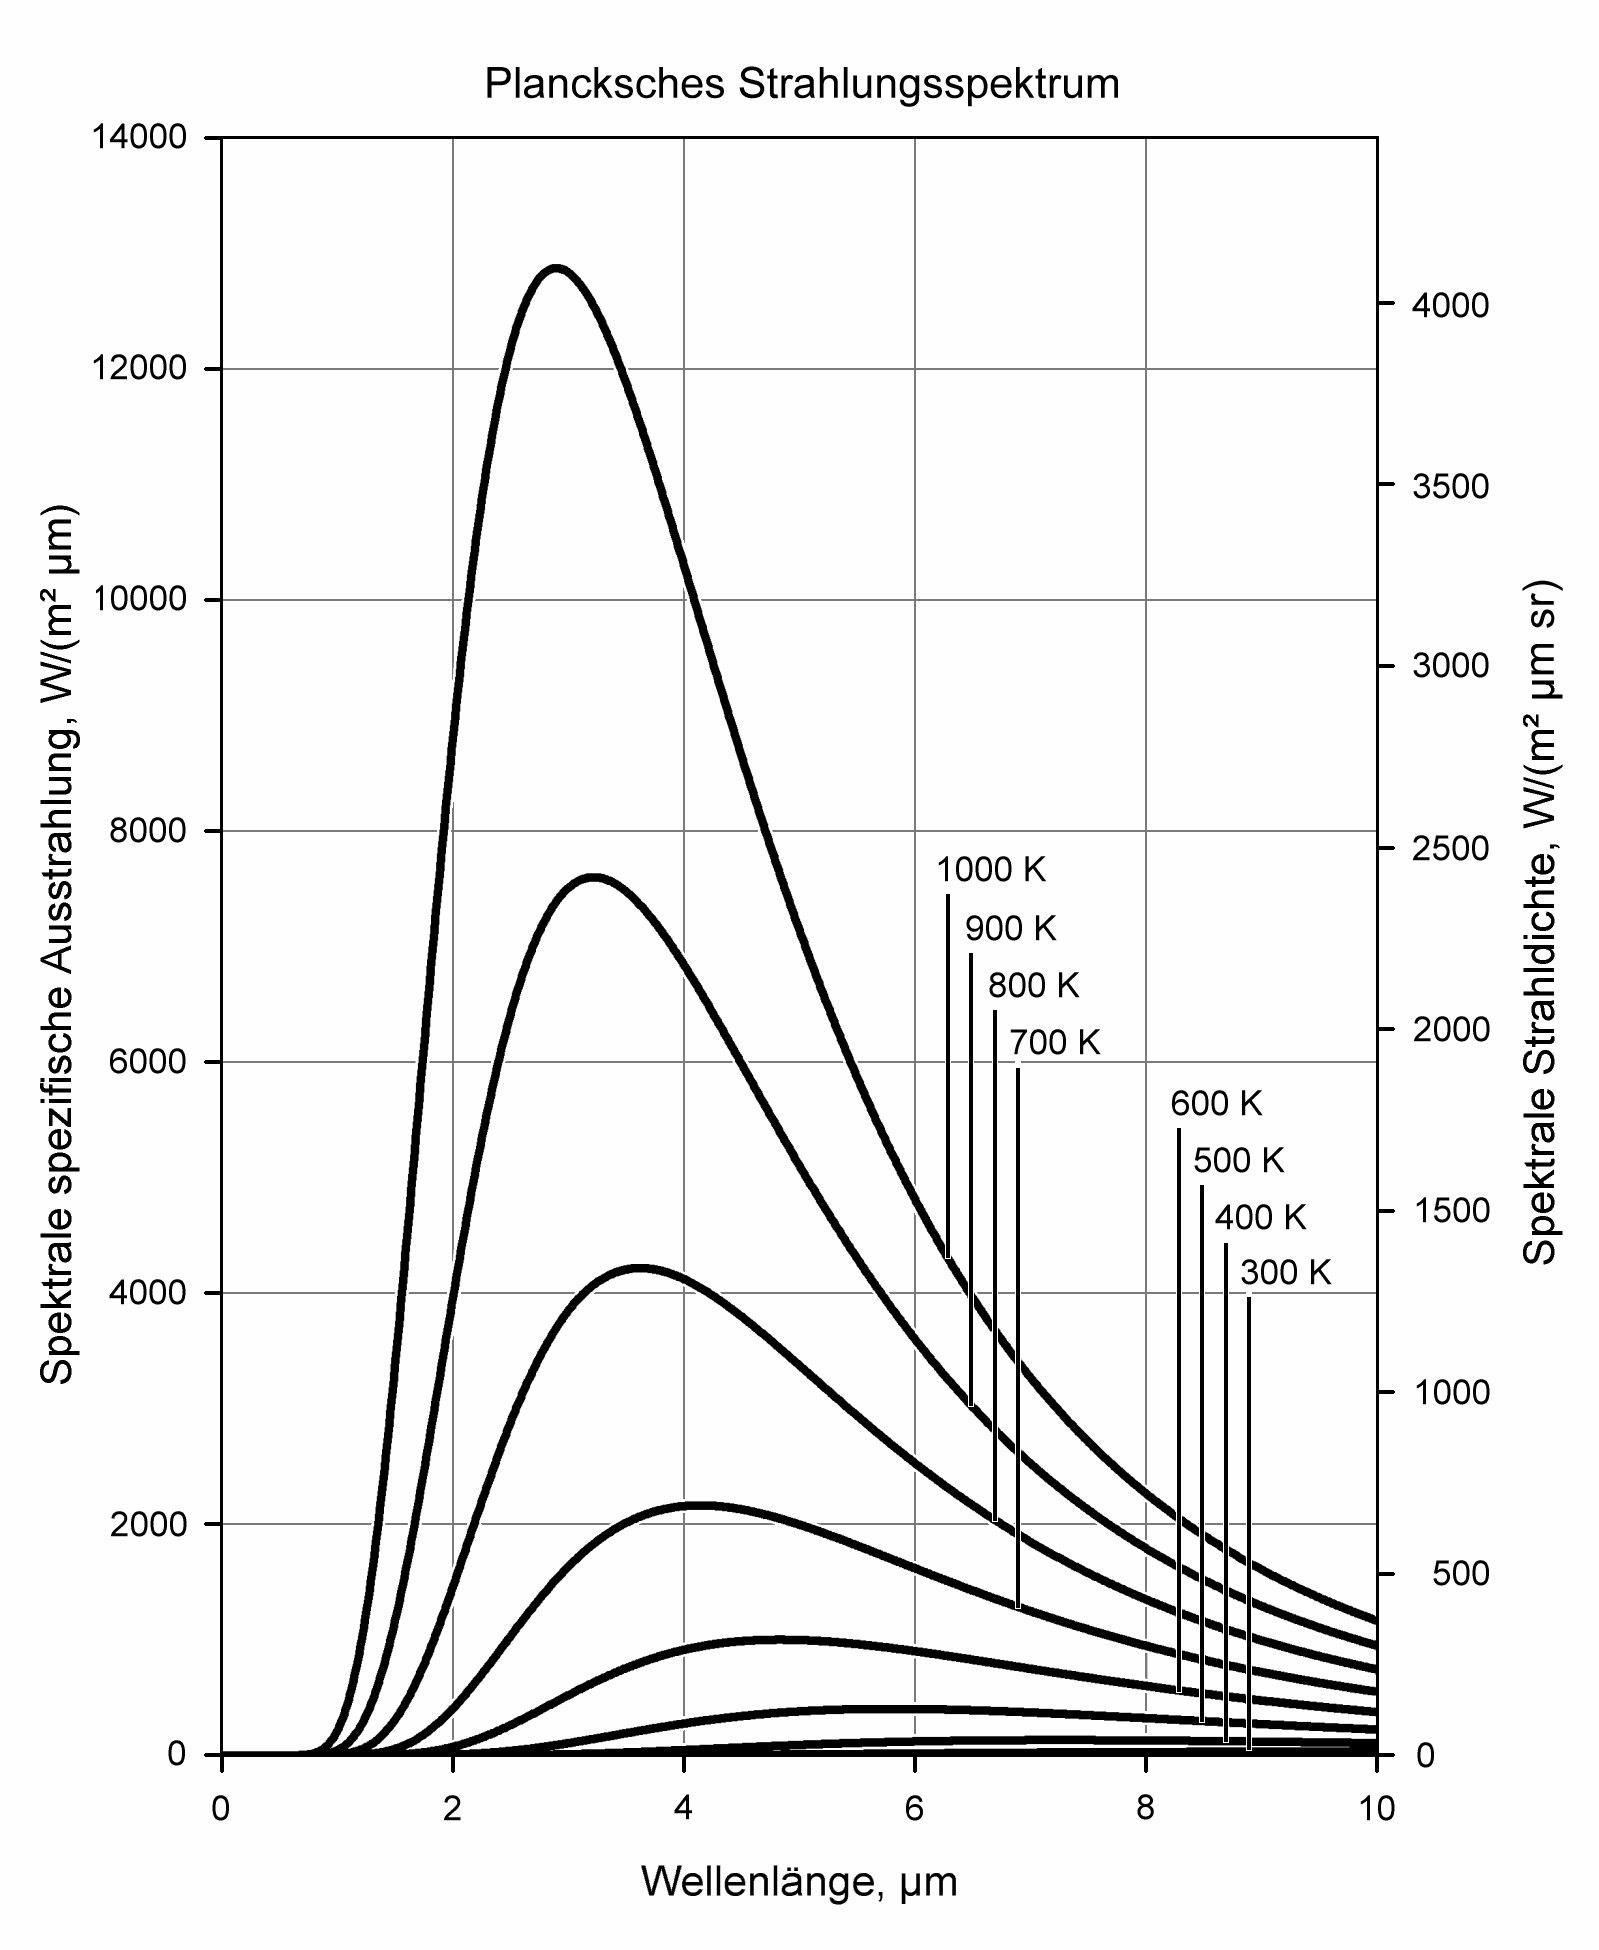
\includegraphics[width=0.5\textwidth]{../media/B1.1/BlackbodySpectrum_lin_150dpi_de.png}
	\caption{Schwarzkörperstrahlung für verschiedene Temperaturen \cite{abb:SpektrumSK}}
	\label{abb:SpektrumSK}
\end{figure}

\hypertarget{strahlungsdichte}{%
\subsubsection{Strahlungsdichte}\label{strahlungsdichte}}

Die Strahldichte oder Strahlungsdichte \(S\) beschreibt die Strahlung, die ein Flächenelement \(\mathrm dA\) eines Strahlers in einen Raumwinkel \(\mathrm d\Omega\) abstrahlt. Sie ist allgemein das Differential der Strahlungsleistung \(\Phi\). \cite{Demtröder,Strahldichte}

\[
\begin{eqnarray}
    S &=& \frac{\mathrm d^2\Phi}{\mathrm dA \cdot \mathrm d\Omega}
\end{eqnarray}
\]

\hypertarget{wiensches-verschiebungsgesetz}{%
\subsubsection{Wien'sches
Verschiebungsgesetz}\label{wiensches-verschiebungsgesetz}}

Das Wien'sche Verschiebungsgesetz beschreibt abhängig von der Temperatur \(T\), bei welcher Wellenlänge \(\hat{\lambda}\) bzw. Frequenz \(\hat{\nu}\) die größte Wärmeleistung abgestrahlt wird. Dadurch beschreibt es die Temperaturabhängigkeit des Maximums des Planck'schen Strahlungsgesetzes \(\eqref{eq:PlackStrahlung}\).

\[
\begin{eqnarray}
    \hat{\lambda}\cdot T &=& 2.898\cdot10^{-3}\mathrm{\,m\cdot K}
        \label{eq:WienLambda}\\
    \hat{\nu}\cdot T &=& 5.879\cdot10^{10} \mathrm{\,m\cdot Hz}
        \label{eq:WienNu}
\end{eqnarray}
\]

\hypertarget{elektrisches-dipolmoment}{%
\subsection{elektrisches Dipolmoment}\label{elektrisches-dipolmoment}}

Das elektrische Dipolmoment \(\vec \mu\) ist das erste Moment aus der Multipolentwicklung einer Ladungsverteilung \(\rho(\vec r)\). \cite{Dipolmoment}
Es ist parallel zum elektrischen Feld \(\vec E\) und beschreibt die Ungleichverteilung von Ladungen.

\[
\begin{eqnarray}
    \vec \mu &=& \int \vec r \rho(\vec r) \,\mathrm d^3\vec r
\end{eqnarray}
\]

\noindent
Atome im Grundzustand haben kein permanentes Dipolmoment, Moleküle können dagegen ein permanentes Dipolmoment haben. Ein Beispiel dafür ist Wasser \((\ce{H_2O})\).

\hypertarget{dipoluxfcbergang}{%
\subsubsection{Dipolübergang}\label{dipoluxfcbergang}}

Um ein Molekül durch die Absorption eines Photons anzuregen, muss ein Dipolübergang stattfinden. Dabei wird der quantenmechanische Zustand des Moleküls gestört, was durch zeitabhängige Störungstheorie beschrieben wird. \cite{Hinderer}

\hypertarget{uxfcbergangsdipolmoment}{%
\subsubsection{Übergangsdipolmoment}\label{uxfcbergangsdipolmoment}}

Die Störung wird als Übergangsdipolmoment \(\vec\mu_{01}\) bezeichnet. Es wird durch den Operator des Dipolmoments \(\hat {\vec \mu}_e\) sowie den Anfangszustand \(\ket{\Psi_0}\) und den Endzustand \(\ket{\Psi_1}\) berechnet. So lange das Übergangsdipolmoment \(\vec\mu_{01}\neq0\) nicht verschwindet, ist der Übergang erlaubt.

\[
\begin{eqnarray}
    \vec \mu_{01} &=& \expval{\Psi_0\left|\hat {\vec \mu}_e\right|\Psi_1}
\end{eqnarray}
\]

\noindent
Je größer das Übergangsdipolmoment ist, desto großer ist auch das Absorptionsvermögen.

\hypertarget{freiheitsgrade}{%
\subsection{Freiheitsgrade}\label{freiheitsgrade}}

Die Zahl der Freiheitsgrade \(f\) gibt an, auf wie viele Arten
beispielsweise ein Gasmolekül Energie speichern kann, z.B. in
Translation entlang einer Koordinatenachse, Rotation oder Schwingungen.

Einatomige Moleküle haben üblicherweise \(3\) Freiheitsgrade durch
Translation. Zweiatomige Moleküle haben zusätzlich noch zwei
Freiheitsgrade durch Rotation, also insgesamt \(5\).

\hypertarget{infrarotaktivituxe4t}{%
\subsection{Infrarotaktivität}\label{infrarotaktivituxe4t}}

\hypertarget{mathematische-grundlagen}{%
\subsection{Mathematische Grundlagen}\label{mathematische-grundlagen}}

\hypertarget{gauuxdfverteilung}{%
\subsubsection{Gaußverteilung}\label{gauuxdfverteilung}}

Die Gaußverteilung entspricht der Wahrscheinlichkeitsdichtefunktion \(\phi_{\mu,\sigma^2}(\chi)\) mit dem Erwartungswert \(\mu\) und der Standardabweichung \(\sigma\). Manchmal wird die Gaußverteilung auch als Normalverteilung bezeichnet, manchmal bezeichnet die Normalverteilung dagegen einen Spezialfall mit \(\mu=\sigma=1\). In Abbildung \ref{abb:gaussians} sind verschiedene Gaußverteilungen dargestellt.

\[
\begin{eqnarray}
    \phi_{\mu,\sigma^2}(\chi) &=&
        \frac{1}{\sqrt{2\pi\sigma^2}}
        \exp\left[
            -
            \frac{(\chi - \mu)^2}{2\sigma^2}
        \right]
\end{eqnarray}
\]

\begin{figure}[h]
	\centering
	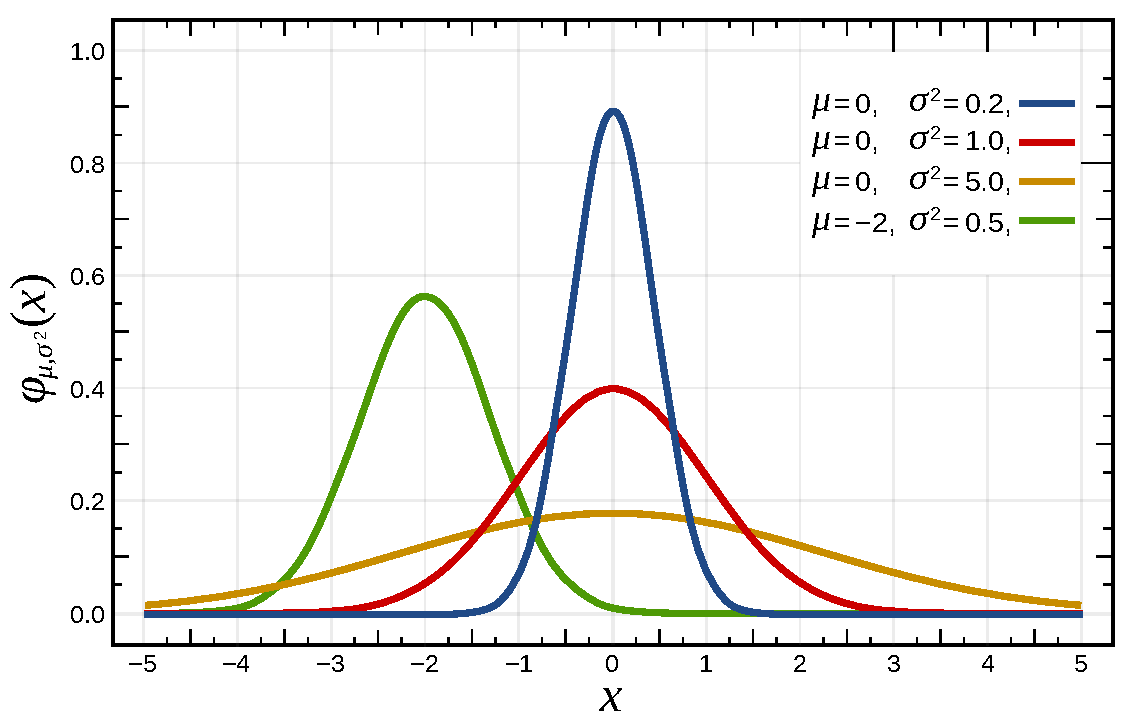
\includegraphics[width=0.7\textwidth]{../media/B1.1/Gaussverteilungen.pdf}
	\caption{Gaußverteilungen mit verschiedenen Parametern \cite{abb:gaussians}}
	\label{abb:gaussians}
\end{figure}

\noindent
Werden Zufallsvariablen gemessen, so haben sie immer eine gewisse Streuung. Nach dem Grenzwertsatz ist diese Streuung gaußverteilt. Bei genügend Messungen kann man annehmen, dass \(68.3\%\) der Zufallsvariablen im Intervall \(\mu\pm\sigma\) liegen.

Im \(2\sigma\)--Intervall werden \(95.4\%\) der Zufallsvariablen erwartet, im \(3\sigma\)--Intervall sogar \(99.7\%\).

\hypertarget{treppenfunktion}{%
\subsubsection{Treppenfunktion}\label{treppenfunktion}}

Eine Treppenfunktion ist eine Funktion, die abschnittsweise aus konstanten Funktionen zusammengesetzt ist.

Sei \(\tau:[a,b]\rightarrow \mathbb R\) eine Treppenfunktion, dann gibt es \(N\) Intervalle \((x_i, x_{i+1})\) und Konstanten \(c_i\), sodass folgende Bedingungen erfüllt sind. \cite{Einsiedler}

\[
\begin{eqnarray}
    x_0 &=& a \\
    x_n &=& b \\
    \forall i:\quad
        x_i &<& x_{i+1} \\
    \forall x\in[x_i, x_{i+1}]:\quad
        \tau(x) &=& c_i
\end{eqnarray}
\]

\noindent
Das Integral über eine Treppenfunktion wird als Summe über die Zerlegung \(\{x_i\}\) gebildet.

\[
\begin{eqnarray}
    \int_a^b\tau(x)\,\mathrm dx
        &=& \sum_{i=0}^N c_i\cdot (x_{i+i}-x_i)
\end{eqnarray}
\]

\hypertarget{numerische-integration}{%
\subsubsection{numerische Integration}\label{numerische-integration}}

Ein Integral \(\int_a^b f\) kann numerisch angenähert werden, indem die Funktion \(f\) durch eine Treppenfunktion dargestellt wird. Diese Methode addiert rechteckige Flächenelemente, es gibt auch ähnliche Methoden mit beispielsweise trapezförmigen Flächenelementen.

Der Integrationsbereich \([a,b]\) wird in \(N\) gleich große Intervalle zerlegt. Dadurch kann die Schrittweite \(\Delta x\) definiert werden. Die Stufenfunktion wird so gewählt, dass die Funktion \(f\) in jedem Teilintervall \((x_i, x_{i+1})\) angenähert wird. Damit kann das Integral ermittelt werden.

\[
\begin{eqnarray}
    \Delta x &=& \frac{b--a}{N} \\
    \forall i:\quad
        f(x) &\approx& f(x+i\cdot\Delta x) \\
    \int_a^b f(x) \,\mathrm dx
        &\approx& \Delta x\cdot
            \sum_{i=1}^N f(x + i\cdot \Delta x)
\end{eqnarray}
\]

\noindent
Dies ist nur eine Annäherung eines echten Integrals, die kein exaktes Ergebnis liefert. Wenn \(\Delta x\) beliebig klein werden könnte, so nähert man sich einem Riemann--Integral an.

\hypertarget{das-lambertbeersche-gesetz}{%
\subsection{Das Lambert--Beer'sche
Gesetz}\label{das-lambertbeersche-gesetz}}

\hypertarget{treibhauseffekt}{%
\subsection{Treibhauseffekt}\label{treibhauseffekt}}

\clearpage
\hypertarget{durchfuxfchrung}{%
\section{Durchführung}\label{durchfuxfchrung}}

\clearpage
\hypertarget{auswertung}{%
\section{Auswertung}\label{auswertung}}

\clearpage
\hypertarget{fazit}{%
\section{Fazit}\label{fazit}}

\clearpage
\hypertarget{literatur}{%
\section{Literatur}\label{literatur}}
\renewcommand{\section}[2]{} % remove extra title
\begin{thebibliography}{9}
\bibitem{UzK}
	Universität zu Köln, ``B1.1: Infrarotabsorption in \(\ce{CO_2}\)'', April 2024
\bibitem{Bakan}
  S. Bakan \& E. Raschke, ``Der natürliche Treibhauseffekt'', Promet 28,
	Deutscher Wetterdienst, 2002, Online verfügbar unter
	\url{https://www.dwd.de/DE/leistungen/pbfb_verlag_promet/pdf_promethefte/28_3_4_pdf.pdf}
\bibitem{Demtröder}
	W. Demtröder, ``Experimentalphysik 3: Atome, Moleküle und Festkörper'',
	Springer--Spektrum--Verlag, 5. Auflage 2016, DOI:
	\href{https://doi.org/10.1007/978-3-662-49094-5}{10.1007/978-3-662-49094-5}
\bibitem{Strahldichte}
	Wikipedia, ``Strahldichte'',
	\url{https://de.wikipedia.org/wiki/Strahldichte}, Abruf am 02.05.2024
\bibitem{abb:SpektrumSK}
	Wikipedia, \url{https://commons.wikimedia.org/wiki/File:BlackbodySpectrum_lin_150dpi_de.png},
	Abruf am 02.05.2024
\bibitem{Dipolmoment}
	Lexikon der Physik, ``Dipolmoment'',
	\url{https://www.spektrum.de/lexikon/physik/elektrisches-dipolmoment/3960},
	Abruf am 02.05.2024
\bibitem{Hinderer}
	F. Hinderer, ``UV/Vis--Absorptions- und Fluoreszenz--Spektroskopie'',
	2020, DOI \href{https://doi.org/10.1007/978-3-658-25441-4}{10.1007/978-3-658-25441-4}
\bibitem{Fließbach}
	T. Fließbach, ``Statistische Physik'', 2018, DOI
	\href{https://doi.org/10.1007/978-3-662-58033-2}{10.1007/978-3-662-58033-2}
\bibitem{abb:gaussians}
	Wikimedia,
	\url{https://commons.wikimedia.org/wiki/File:Normal_Distribution_PDF.svg},
	2023-02-23
\bibitem{Einsiedler}
	M. Einsiedler, ``Analysis I: Kapitel \(1\)-\(9\)'', 2022,
	\url{https://wp-prd.let.ethz.ch/analysis19/chapter/treppenfunktionen-und-deren-integral},
	Abruf am 03.05.2024
\end{thebibliography}
\end{document}
